\section{Introduction}
Many forms of nature exhibit the properties of fractals [\cite{Mandlebrot}]; being self-similar on different length scales, where conventional geometry is inappropriate. Their presence is known in nonlinear optics [\cite{Soljacic, Segev}]. Fractal architecture has interest in applications such as the design of antennas [\cite{Radonic,Puente-Baliarda,Siakavara}], image compressing [\cite{Jacquin}] and references therein. Waves that have encountered fractals are known as diffractals [\cite{Berry}]. Diffractals showing redundancy/robustness [\cite{Verma,Verma2}].


\section{Theory}
How fractals are generated. Sierpinski carpets can be generated using the iteration [\cite{Allouche,Velez}]:
\begin{equation}
\Bigg\{0\rightarrow \Bigg[\begin{array}{ccc}
0 & 0 & 0 \\
0 & 0 & 0\\
0 & 0 & 0\end{array}\Bigg], 1\rightarrow\Bigg[\begin{array}{ccc}
1 & 1 & 1 \\
1 & 0 & 1\\
1 & 1 & 1\end{array}\Bigg] \Bigg\}
\end{equation}
This can be implemented analytically using the Kronecker tensor product of the base matrix, $\Big[\begin{smallmatrix} 1 & 1 & 1 \\ 1 & 0 & 1\\ 1 & 1 & 1\end{smallmatrix}\Big]$, with itself, to create a fractal of increasing order the Kronecker tensor product can be applied to the matrix with the base matrix. The number of times this operation is performed determines the fractal order. This method can be applied to any base matrix to produce a matrix with fractal architecture.\\
Interestingly, the diffraction pattern of fractal apertures is also a self-similar fractal [\cite{Horvath,Hou,Skigin}]. Analytically, to look at the diffraction pattern of an aperture in the far-field approximation the Fourier transform of the aperture is to be taken [\cite{Scott1,Scott2}]. This can be proven analytically using the scaling and shifting properties of the Fourier transform. Let our base matrix take the form $f(x,y)$, and it's Fourier transform $\mathcal{F}[f(x,y)] = F(x,y)$. A fractal can be considered a superposition of the base matrix scaled and shifted many times, $\sum_i f(a_ix-b_i,c_iy-d_i)$. Taking the Fourier transform we get the result:
\begin{equation}
\begin{split}
\mathcal{F}\Big[\sum_if(a_ix&-b_i,c_iy-d_i)\Big] = \sum_i\int_{-\infty}^{\infty}\int_{-\infty}^{\infty}f(a_ix-b_i,c_iy-d_i)\exp[-2\pi i(k_xx+k_yy)]dxdy\\
&= \sum_i\int_{-\infty}^{\infty}\int_{-\infty}^{\infty} \frac{f(u,v)}{a_ic_i}\exp[-2\pi i(\frac{k_xu}{a_i}+k_xb_i+\frac{k_yv}{c_i}+k_yd_i)]dudv\\
&=\sum_i\exp[-2\pi i(k_xb_i+k_yd_i)]\int_{-\infty}^{\infty}\int_{-\infty}^{\infty} \frac{f(u,v)}{a_ic_i}\exp[-2\pi i(\frac{k_xu}{a_i}+\frac{k_y v}{c_i})]dudv\\
&=\sum_i\exp[-2\pi i(k_xb_i+k_yd_i)]\frac{F(\frac{x}{a_i},\frac{y}{c_i})}{|a_i||c_i|}
\end{split}
\end{equation}
\begin{figure}[!ht]
\includegraphics[width=\textwidth]{FTFractal.pdf}
\caption{a) Sierpinski carpet of fractal order 7, b) the Fourier transform of the Sierpinski carpet, c) an arbitrary subsection of the Fourier transform. In b) and c) a logarithmic scale is used to show detail.}
\label{FTFractal}
\end{figure}
 Figure \ref{FTFractal} shows that the Fourier transform of a fractal aperture also exhibits fractal architecture, a repeating pattern that displays at every length scale.\\
 Since the Fourier transform of the fractal function also has the same scaled and shifted properties the Fourier transform is also exhibits fractal architecture.\\
\textit{Show fractal dimension relates between the aperture and the diffraction pattern} [\cite{Guerin,Allain,Dubuc}].\\
A box-counting method can be used to estimate the capacity dimension fractal structures [\cite{McMullen,Sagan,Falconer}]. After $n$ iterations the total number of boxes needed to cover the structure is $N_n$ and the smallest length of a box is $L_n$. This results in a general formulation for the dimension of a structure:
\begin{equation}
 d_f = -\lim_{n\rightarrow\infty}\frac{\log N_n}{\log L_n}
\end{equation} 
For the case of Sierpinski carpets the number of boxes remaining is $N_n = 8^n$ and the length of the smallest box is $L_n = 3^{-n}$ since the base matrix is a $3\times 3$ matrix with $8$ nonzero entries. As $n$ tends to infinity, and the size of the boxes tends to zero, the dimension of Sierpinski carpet becomes:
\begin{equation}
\begin{split}
d_f &= -\lim_{n\rightarrow\infty}\frac{\log 8^n}{\log 3^{-n}}\\
&=\lim_{n\rightarrow\infty}\frac{n\log 8}{n\log 3}\\
&=\frac{3\log 2}{\log 3}\\
&=1.8927892607143721...
\end{split}
\end{equation}
To compare the fractal dimensions between Sierpinski carpets of different orders a box length of size $\epsilon$ is used. As the fractal order increases by $n$ the fractal dimension reduces by the factor 
\begin{equation}
K = \frac{\log((\frac{8}{9})^{-n})}{\log 1/\epsilon}
\end{equation}
In this Letter we show that because of the self-similarity at different length scales the original image can be reconstructed from subsets it's Fourier transform. The reconstruction can be found by taking the inverse Fourier transform of any subset. 
\begin{figure}[b!]
\includegraphics[width=\textwidth]{AnalyticalHolgramReconstruction.pdf}
\caption{Holograms of Sierpinski carpets of different orders and their reconstructions from an arbitrary 1\% subset of the Fourier transform.}
\label{AnalRecon}
\end{figure}
Figure \ref{AnalRecon} shows the Sierpinski carpet holograms at different fractal orders and their corresponding reconstructions from a 1\% subset of the Fourier transform. As the fractal order increases the reconstruction from the subset better resembles the original image. The subset of the Fourier transformed image used to reconstruct the image is irrelevant, the image can be reconstructed if the fractal order ids high enough.\\
Experimentally, Fourier optics can be used to model the diffraction profile generated from an aperture at the focal plane when using an imaging lens [\cite{Goodman}]. In the field of the focal plane of an imaging lens the complex amplitude distribution corresponds to the Fraunhofer diffraction pattern of the field incident on the lens. We will use a lens to compute the experimental equivalent of the Fourier transform. An aperture will take a subset of the diffraction profile and another focusing lens will take the inverse Fourier transform.
%\begin{figure}[!ht]
%\includegraphics[width=\textwidth]{method.pdf}
%\caption{a) Sierpinski carpet of fractal order 7, b) the Fourier transform of the Sierpinski carpet, c) an arbitrary subsection of the Fourier transform. In b) and c) a logarithmic scale is used to show detail}
%\label{FTFractal}
%\end{figure}

%
%\begin{figure}[htbp]
%%\centering\includegraphics[width=7cm]{opexfig1}
%\caption{Sample caption (Ref. \cite{Oron03}, Fig. 2).}
%\end{figure}
%
%\begin{equation}
%H = \frac{1}{2m}(p_x^2 + p_y^2) + \frac{1}{2} M{\Omega}^2
%     (x^2 + y^2) + \omega (x p_y - y p_x).
%\end{equation}

\section{Results}
Figure \ref{ExpSetup} shows the experimental setup for creating fractal apertures and observing the corresponding diffraction pattern and reconstructed image. A $4f$ optical arrangement is used as a tool for optical information processing in Fourier optics. A 632.8nm coherent laser source is spatially filtered, then expanded and collumated to illuminate the full area of a 800x600 pixel spatial light modulator (SLM). The 4f system is composed of 2 $5cm$ lenses placed after the SLM. The first lens Fourier transforms the fractal aperture at the focal plane. An aperture is placed at the focal plane that only accepts a small window of the Fourier transformed fractal aperture through. The second lens acts to take the inverse Fourier transform to reconstruct the aperture.
\begin{figure}[!ht]
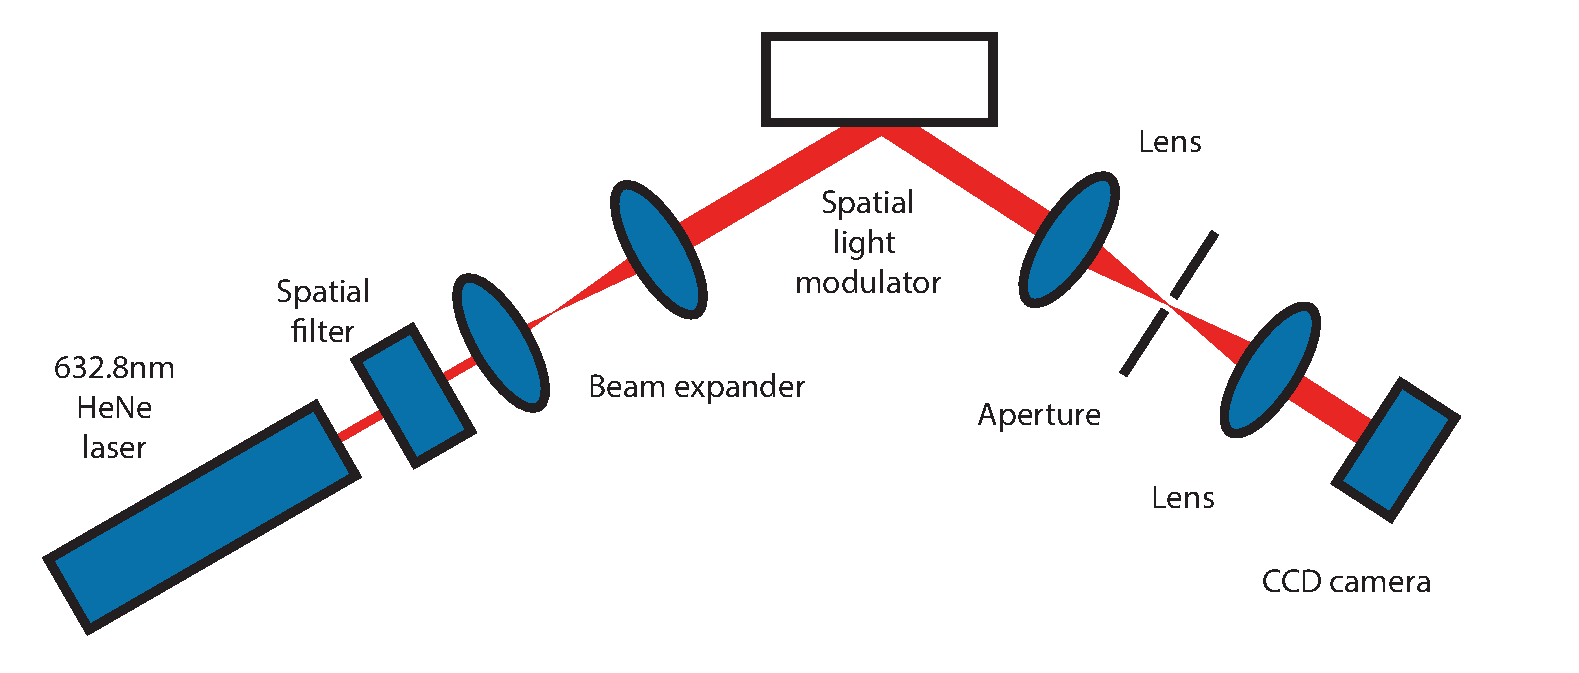
\includegraphics[width=\textwidth]{ExpSetup2.pdf}
\caption{Experimental Setup}
\label{ExpSetup}
\end{figure}

\begin{figure}[h!t]
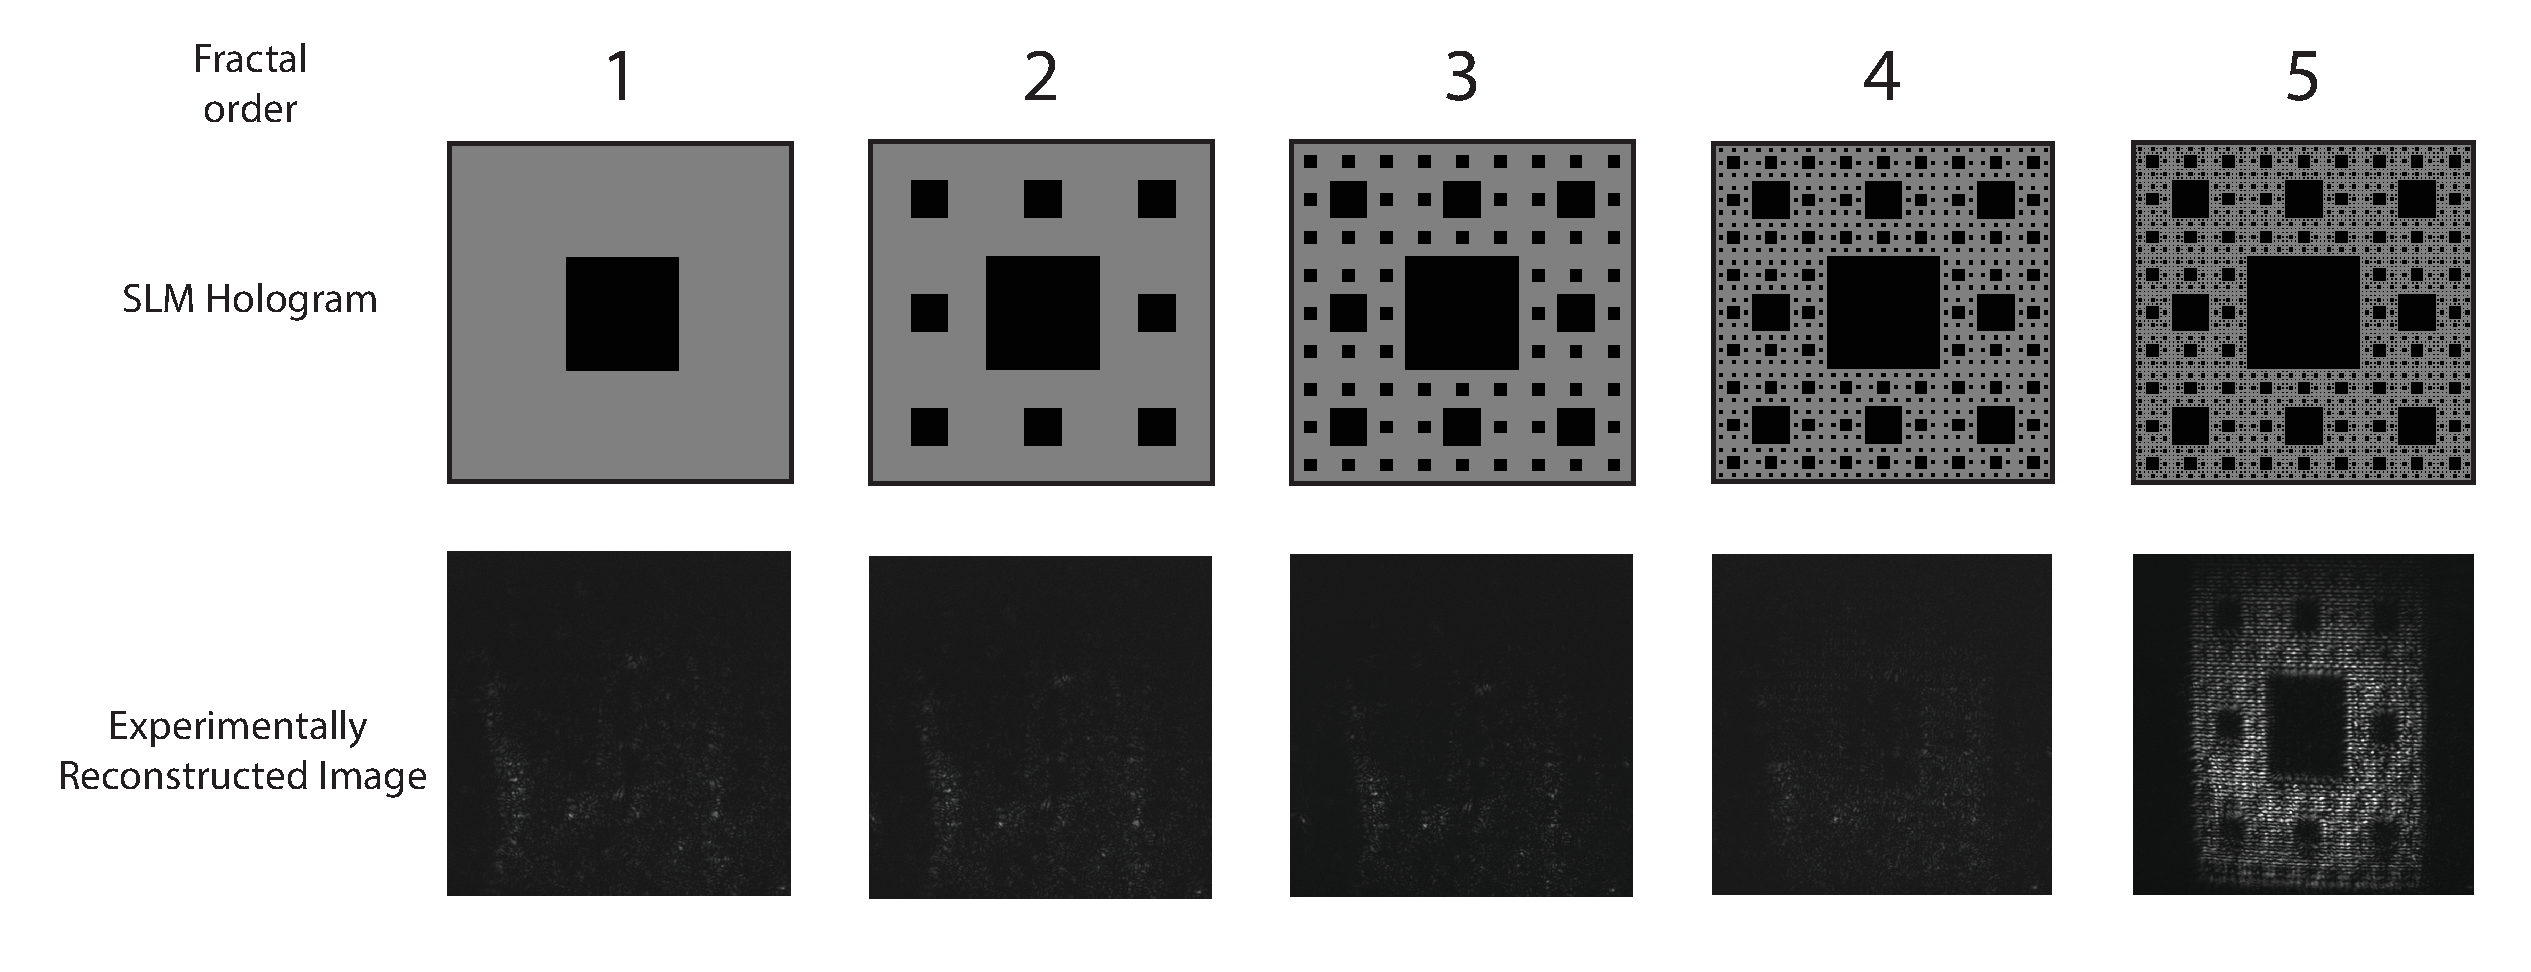
\includegraphics[width=\textwidth]{ExperimentallHolgramReconstruction.pdf}
\caption{Sample caption .}
\label{Recon}
\end{figure}
%\subsection*{Other graphs to possibly add}
%Graph showing how small subset of image is needed to recreate original signal, i.e. area of subset on x-axis, some sort of quality factor of recreation on the y-axis.\\
\section{Discussion}
\subsection{Spatial Multiplexing}
Any image, if given fractal architecture can exhibit the same transmission properties and can provide the basis of spatial multiplexing. If we consider a $3\times 3$ base matrix composed of ones and zeros, there is $2^9 = 512$, 9-bit, possible variants, for a $4\times 4$ matrix, there are $2^16 = 65,536$, 16-bit, possible variants. If these base matrices are given fractal architecture by repeating the matrix on different length scales.\\
Figure \ref{Multiplex} shows 5 examples of 9-bit patterns in a $3\times 3 $ array can be converted to a fractal for optical multiplexing. Here the Sierpinski carpet is one variant, beginning with one particular base matrix, $\Big[\begin{smallmatrix} 1 & 1 & 1 \\ 1 & 0 & 1\\ 1 & 1 & 1\end{smallmatrix}\Big]$. Figure \ref{Recon} shows 5 different variants, a) with base matrix  $\Big[\begin{smallmatrix} 1 & 0 & 1 \\ 1 & 1 & 1\\ 1 & 0 & 1\end{smallmatrix}\Big]$, b) with base  $\Big[\begin{smallmatrix} 1 & 1 & 0 \\ 0 & 1 & 1\\ 0 & 1 & 1\end{smallmatrix}\Big]$, c) with base matrix  $\Big[\begin{smallmatrix} 1 & 1 & 0 \\ 1 & 0 & 0\\ 1 & 1 & 1\end{smallmatrix}\Big]$, d) with base matrix  $\Big[\begin{smallmatrix} 1 & 0 & 0 \\ 1 & 1 & 0\\ 1 & 1 & 1\end{smallmatrix}\Big]$, and e) with base matrix  $\Big[\begin{smallmatrix} 1 & 1 & 0 \\ 1 & 1 & 1\\ 1 & 1 & 1\end{smallmatrix}\Big]$.\\
It is important to note that the reconstructions can only work when the base matrices are converted to fractals, here by computing the Kronecker tensor product of the base matrix with itself many times over. When the reconstruction is attempted with the base matrix itself, only by taking the full Fourier transform can the original image be reconstructed; if a subset is taken in the Fourier plane the original image cannot be reconstructed. \\
From the reconstructed image, the original can be regenerated using a simple threshold function. Dividing the reconstructed image into a $3\times 3$ array and measuring the intensity in each element, if it is above a certain threshold value, that element is assigned a value of 1, if below the element is assigned a value 0. Once all elements in the $3\times 3$ array is complete it should parallel the base matrix.
\begin{figure}[!ht]
\includegraphics[width=\textwidth]{Multiplexing.pdf}
\caption{5 Examples of possible 512 9-bit patterns, their fractal architecture holograms are shown with their corresponding reconstructions}
\label{Multiplex}
\end{figure}
\section{Conclusion}
In conclusion we have shown how transmission signals can be multiplexed using a fractal basis. This technique allows large quantities of data to be transferred and reconstructed from a small subset of the projected diffractal. This work has applications in data transmission and other areas.